\documentclass[journal,12pt,twocolumn]{IEEEtran}
%
\usepackage{setspace}
\usepackage{textcomp}
\usepackage{gensymb}
\usepackage{xcolor}
\usepackage{caption}
%\usepackage{subcaption}
%\doublespacing
\singlespacing

%\usepackage{graphicx}
%\usepackage{amssymb}
%\usepackage{relsize}
\usepackage[cmex10]{amsmath}
\usepackage{mathtools}
%\usepackage{amsthm}
%\interdisplaylinepenalty=2500
%\savesymbol{iint}
%\usepackage{txfonts}
%\restoresymbol{TXF}{iint}
%\usepackage{wasysym}
\usepackage{hyperref}
\usepackage{amsthm}
\usepackage{mathrsfs}
\usepackage{txfonts}
\usepackage{stfloats}
\usepackage{cite}
\usepackage{cases}
\usepackage{subfig}
%\usepackage{xtab}
\usepackage{longtable}
\usepackage{multirow}
%\usepackage{algorithm}
%\usepackage{algpseudocode}
%\usepackage{enumerate}
\usepackage{enumitem}
\usepackage{mathtools}
%\usepackage{iithtlc}
%\usepackage[framemethod=tikz]{mdframed}
\usepackage{listings}
\let\vec\mathbf
\usepackage{tikz}
\usetikzlibrary{shapes, arrows, positioning}
\usepackage[RPvoltages]{circuitikz}

%\usepackage{stmaryrd}


%\usepackage{wasysym}
%\newcounter{MYtempeqncnt}
\DeclareMathOperator*{\Res}{Res}
%\renewcommand{\baselinestretch}{2}
\renewcommand\thesection{\arabic{section}}
\renewcommand\thesubsection{\thesection.\arabic{subsection}}
\renewcommand\thesubsubsection{\thesubsection.\arabic{subsubsection}}

\renewcommand\thesectiondis{\arabic{section}}
\renewcommand\thesubsectiondis{\thesectiondis.\arabic{subsection}}
\renewcommand\thesubsubsectiondis{\thesubsectiondis.\arabic{subsubsection}}

%\renewcommand{\labelenumi}{\textbf{\theenumi}}
%\renewcommand{\theenumi}{P.\arabic{enumi}}

% correct bad hyphenation here
\hyphenation{op-tical net-works semi-conduc-tor}

\lstset{
language=Python,
frame=single, 
breaklines=true,
columns=fullflexible
}



\begin{document}
\theoremstyle{definition}
\newtheorem{theorem}{Theorem}[section]
\newtheorem{problem}{Problem}
\newtheorem{proposition}{Proposition}[section]
\newtheorem{lemma}{Lemma}[section]
\newtheorem{corollary}[theorem]{Corollary}
\newtheorem{example}{Example}[section]
\newtheorem{definition}{Definition}[section]
%\newtheorem{algorithm}{Algorithm}[section]
%\newtheorem{cor}{Corollary}
\newcommand{\BEQA}{\begin{eqnarray}}
\newcommand{\EEQA}{\end{eqnarray}}
\newcommand{\define}{\stackrel{\triangle}{=}}
\newcommand{\myvec}[1]{\ensuremath{\begin{pmatrix}#1\end{pmatrix}}}
\newcommand{\mydet}[1]{\ensuremath{\begin{vmatrix}#1\end{vmatrix}}}

\bibliographystyle{IEEEtran}
%\bibliographystyle{ieeetr}

\providecommand{\nCr}[2]{\,^{#1}C_{#2}} % nCr
\providecommand{\nPr}[2]{\,^{#1}P_{#2}} % nPr
\providecommand{\mbf}{\mathbf}
\providecommand{\pr}[1]{\ensuremath{\Pr\left(#1\right)}}
\providecommand{\qfunc}[1]{\ensuremath{Q\left(#1\right)}}
\providecommand{\sbrak}[1]{\ensuremath{{}\left[#1\right]}}
\providecommand{\lsbrak}[1]{\ensuremath{{}\left[#1\right.}}
\providecommand{\rsbrak}[1]{\ensuremath{{}\left.#1\right]}}
\providecommand{\brak}[1]{\ensuremath{\left(#1\right)}}
\providecommand{\lbrak}[1]{\ensuremath{\left(#1\right.}}
\providecommand{\rbrak}[1]{\ensuremath{\left.#1\right)}}
\providecommand{\cbrak}[1]{\ensuremath{\left\{#1\right\}}}
\providecommand{\lcbrak}[1]{\ensuremath{\left\{#1\right.}}
\providecommand{\rcbrak}[1]{\ensuremath{\left.#1\right\}}}
\providecommand{\rect}[1]{\text{rect}\ensuremath{\left(#1\right)}}
\providecommand{\sinc}[1]{\text{sinc}\ensuremath{\left(#1\right)}}
\theoremstyle{remark}
\newtheorem{rem}{Remark}
\newcommand{\sgn}{\mathop{\mathrm{sgn}}}
\providecommand{\abs}[1]{\left\vert#1\right\vert}
\providecommand{\res}[1]{\Res\displaylimits_{#1}} 
\providecommand{\norm}[1]{\lVert#1\rVert}
\providecommand{\mtx}[1]{\mathbf{#1}}
\providecommand{\mean}[1]{E\left[ #1 \right]}
\providecommand{\fourier}{\overset{\mathcal{F}}{ \rightleftharpoons}}
\providecommand{\ztrans}{\overset{\mathcal{Z}}{ \rightleftharpoons}}

%\providecommand{\hilbert}{\overset{\mathcal{H}}{ \rightleftharpoons}}
%\providecommand{\system}{\overset{\mathcal{H}}{ \longleftrightarrow}}
\providecommand{\system}[1]{\overset{\mathcal{#1}}{ \longleftrightarrow}}
	%\newcommand{\solution}[2]{\textbf{Solution:}{#1}}
\newcommand{\solution}{\noindent \textbf{Solution: }}
\providecommand{\dec}[2]{\ensuremath{\overset{#1}{\underset{#2}{\gtrless}}}}
\numberwithin{equation}{section}
%\numberwithin{equation}{subsection}
%\numberwithin{problem}{subsection}
%\numberwithin{definition}{subsection}
\makeatletter
\@addtoreset{figure}{problem}
\makeatother

\let\StandardTheFigure\thefigure
%\renewcommand{\thefigure}{\theproblem.\arabic{figure}}
\renewcommand{\thefigure}{\theproblem}


%\numberwithin{figure}{subsection}

\def\putbox#1#2#3{\makebox[0in][l]{\makebox[#1][l]{}\raisebox{\baselineskip}[0in][0in]{\raisebox{#2}[0in][0in]{#3}}}}
     \def\rightbox#1{\makebox[0in][r]{#1}}
     \def\centbox#1{\makebox[0in]{#1}}
     \def\topbox#1{\raisebox{-\baselineskip}[0in][0in]{#1}}
     \def\midbox#1{\raisebox{-0.5\baselineskip}[0in][0in]{#1}}

\vspace{3cm}

\title{ 
%\logo{
%}
Fourier Series
%	\logo{Octave for Math Computing }
}
%\title{
%	\logo{Matrix Analysis through Octave}{\begin{center}\includegraphics[scale=.24]{tlc}\end{center}}{}{HAMDSP}
%}


% paper title
% can use linebreaks \\ within to get better formatting as desired
%\title{Matrix Analysis through Octave}
%
%
% author names and IEEE memberships
% note positions of commas and nonbreaking spaces ( ~ ) LaTeX will not break
% a structure at a ~ so this keeps an author's name from being broken across
% two lines.
% use \thanks{} to gain access to the first footnote area
% a separate \thanks must be used for each paragraph as LaTeX2e's \thanks
% was not built to handle multiple paragraphs
%

\author{ G V V Sharma$^{*}$} %<-this  stops a space
%\thanks{*The author is with the Department
%of Electrical Engineering, Indian Institute of Technology, Hyderabad
%502285 India e-mail:  gadepall@iith.ac.in.  All content in the manuscript is 
%released under GNU GPL.  Free to use for anything. }% <-this % stops a space
%\thanks{J. Doe and J. Doe are with Anonymous University.}% <-this % stops a space
%\thanks{Manuscript received April 19, 2005; revised January 11, 2007.}}
%}
% note the % following the last \IEEEmembership and also \thanks - 
% these prevent an unwanted space from occurring between the last author name
% and the end of the author line. i.e., if you had this:
% 
% \author{....lastname \thanks{...} \thanks{...} }
%                     ^------------^------------^----Do not want these spaces!
%
% a space would be appended to the last name and could cause every name on that
% line to be shifted left slightly. This is one of those "LaTeX things". For
% instance, "\textbf{A} \textbf{B}" will typeset as "A B" not "AB". To get
% "AB" then you have to do: "\textbf{A}\textbf{B}"
% \thanks is no different in this regard, so shield the last } of each \thanks
% that ends a line with a % and do not let a space in before the next \thanks.
% Spaces after \IEEEmembership other than the last one are OK (and needed) as
% you are supposed to have spaces between the names. For what it is worth,
% this is a minor point as most people would not even notice if the said evil
% space somehow managed to creep in.



% The paper headers
%\markboth{Journal of \LaTeX\ Class Files,~Vol.~6, No.~1, January~2007}%
%{Shell \MakeLowercase{\textit{et al.}}: Bare Demo of IEEEtran.cls for Journals}
% The only time the second header will appear is for the odd numbered pages
% after the title page when using the twoside option.
% 
% *** Note that you probably will NOT want to include the author's ***
% *** name in the headers of peer review papers.                   ***
% You can use \ifCLASSOPTIONpeerreview for conditional compilation here if
% you desire.




% If you want to put a publisher's ID mark on the page you can do it like
% this:
%\IEEEpubid{0000--0000/00\$00.00~\copyright~2007 IEEE}
% Remember, if you use this you must call \IEEEpubidadjcol in the second
% column for its text to clear the IEEEpubid mark.



% make the title area
\maketitle

\hbadness = 10000, \vbadness = 10000
%\newpage

\tableofcontents

%\renewcommand{\thefigure}{\thesection.\theenumi}
%\renewcommand{\thetable}{\thesection.\theenumi}

\renewcommand{\thefigure}{\theenumi}
\renewcommand{\thetable}{\theenumi}

%\renewcommand{\theequation}{\thesection}


\bigskip

\begin{abstract}
This manual provides a simple introduction to Fourier Series
\end{abstract}
\section{Periodic Function}
Let 
\begin{align}
	x(t) &= A_0\abs{\sin\brak{2\pi f_0 t}}
	\label{eq:10-orig-diff-def}
\end{align}
\begin{enumerate}[label=\thesection.\arabic*
,ref=\thesection.\theenumi]

\item Plot $x(t)$. \\
\solution \\
Download the following python code for the plot of $x(t)$
\begin{lstlisting}
	wget 1_1.py
\end{lstlisting}
\begin{figure}[!ht]
	\centering
	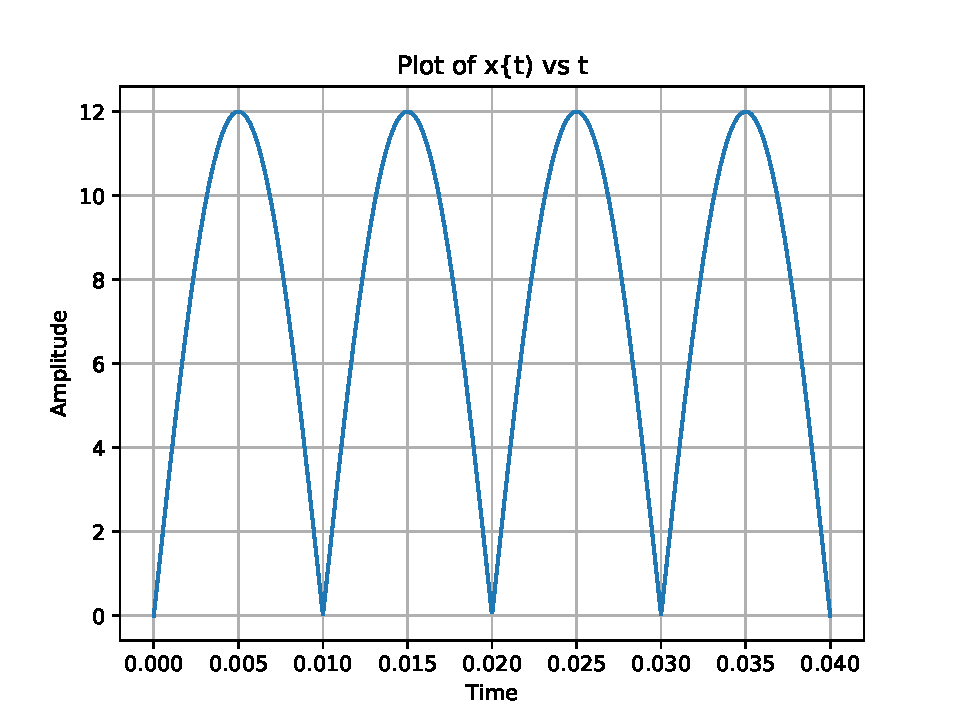
\includegraphics[width=\columnwidth]{figs/1_1.pdf}
	\caption{}
	\label{fig:x(t)}
\end{figure}


\item Show that $x(t)$ is periodic and find its period.
\solution 
\begin{align}
	x(t + T) &= A_{0} \abs{\sin{\brak{2 \pi f_0 (t + T)}}} \\
		 &= A_{0} \abs{\sin{\brak{2 \pi f_0 t + 2 \pi f_0 T}}} 
\end{align}
If $x(t)$ is periodic, then $ x(t) = x(t + T)$
\begin{align}
	x(t) &= A_{0} \abs{sin\brak{2 \pi f_0 (t + T)}} \\
	\abs{\sin{\brak{2 \pi f_0 t}}} &= \abs{\sin{\brak{2 \pi f_0 t + 2 \pi f_0 T)}}} \\
	2 \pi f_0 T &= n \pi \\
		    &T = \frac{n}{f_0} \quad n = 1, 2, \dots 
\end{align}
Fundamental period is
\begin{align}
	T = \frac{1}{2 f_0}
\end{align}

\end{enumerate}


\section{Fourier Series}
Consider $A_0 =12$ and $f_0 = 50$ for all numerical calculations.
\begin{enumerate}[label=\thesection.\arabic*,ref=\thesection.\theenumi]
\item If
\begin{align}
	x(t) = \sum_{k = -\infty}^{\infty}c_ke^{j 2 \pi kf_0 t}
\label{eq:one-Z-complex}
\end{align}
show that 
\begin{align}
	c_k = f_0\int_{-\frac{1}{2f_0}}^{\frac{1}{2f_0}}x(t)e^{-j 2 \pi kf_0 t}\, dt
\label{eq:one-Z}
\end{align}
\solution
\begin{align}
	x(t)e^{-j 2 \pi nf_0t} &= \sum_{k = -\infty}^{\infty}c_ke^{-j 2 \pi (n - k)f_0 t} \\
	\implies &\int_{-\frac{1}{2f_0}}^{\frac{1}{2f_0}} x(t)e^{-j 2 \pi nf_0t} \, {dt} \\ &= \sum_{k = -\infty}^{\infty} c_k \int_{-\frac{1}{2f_0}}^{\frac{1}{2f_0}} e^{-j 2 \pi (n - k)f_0 t} \, {dt} 
\end{align}
But 
\begin{align}
	\int_{-\frac{1}{2f_0}}^{\frac{1}{2f_0}} e^{-2 \pi j (n - k)f_0 t} \,{dt} &=
	\begin{cases}
		\frac{1}{f_0} & k = n \\
		0 & k \ne n	
	\end{cases}	\\
	&= \frac{1}{f_0} \delta(n-k)
\end{align}
\begin{align}
	&\sum_{k = -\infty}^{\infty} c_k \int_{-\frac{1}{2f_0}}^{\frac{1}{2f_0}} e^{-2 \pi j (n - k)f_0 t} \, {dt} \\ &= \sum_{k = -\infty}^{\infty} \frac{c_k \, \delta(n-k)}{f_0} \\
		&= \frac{c_n}{f_0} 
\end{align}
Therefore
\begin{align}
	c_k = f_0\int_{-\frac{1}{2f_0}}^{\frac{1}{2f_0}}x(t)e^{- 2 \pi k j f_0 t}\, {dt}
\end{align}


\item Find $c_k$ for 
\eqref{eq:10-orig-diff-def}
\solution
\begin{align}
c_k = f_0\int_{-\frac{1}{2f_0}}^{\frac{1}{2f_0}}A_0\abs{\sin\brak{2\pi f_0 t}}e^{-2 \pi j kf_0 t}\, dt
\end{align}
\begin{multline}
c_k = f_0\int_{-\frac{1}{2f_0}}^{0}A_0\brak{-\sin\brak{2\pi f_0 t}}e^{-2 \pi j kf_0 t}\,dt \\ +f_0 \int_{0}^{\frac{1}{2f_0}}A_0\brak{\sin\brak{2\pi f_0 t}}e^{-2 \pi j kf_0 t}\, dt
\end{multline}
\begin{multline}
c_k = f_0\int_{0}^{\frac{1}{2f_0}}A_0\sin\brak{2\pi f_0 t}e^{2\pi j kf_0 t}\, dt \\ +f_0\int_{0}^{\frac{1}{2f_0}}A_0\sin\brak{2\pi f_0 t}e^{-2 \pi j kf_0 t}\, dt
\end{multline}
\begin{align}
c_k &= f_0 \int_{0}^{\frac{1}{2f_0}} A_0\sin\brak{2\pi f_0 t} \brak{e^{2 \pi j kf_0 t} + e^{-2 \pi j kf_0 t}} \\
&= f_0A_0 \int_{0}^{\frac{1}{2f_0}} 2\sin\brak{2\pi f_0 t} \cos\brak{2\pi k f_0 t} \, dt 
\end{align}
\begin{multline}
	= f_0A_0 \int_{0}^{\frac{1}{2f_0}} \brak{\sin{\brak{2\pi(1+k)f_0t}}} \\
	+ \int_{0}^{\frac{1}{2 f_0}} \sin{\brak{2\pi(1-k)f_0t}}   
\end{multline}
\begin{align}
\begin{split}
	= {} -f_0A_0 \, &\Bigg[ \frac{\cos\brak{2\pi(1+k)f_0t}}{2\pi(1+k)f_0} + \\ &\frac{\cos\brak{2\pi(1-k)f_0t}}{2\pi(1-k)f_0} \Bigg]
\end{split}
\end{align}
\begin{align}
&= \frac{f_0A_0}{2\pi f_0} \sbrak{\frac{1-(-1)^{1+k}}{1+k} + \frac{1-(-1)^{1-k}}{1-k}} \\
&= \frac{A_0}{2 \pi} \brak{1 + (-1)^k}  \sbrak{\frac{1}{1+k} + \frac{1}{1-k}} \\
&= \brak{1 + (-1)^k} \frac{A_0}{\pi(1-k^2)}
\end{align}
Therefore
\begin{align}
c_k = 
\begin{cases}
	\frac{2A_0}{\pi(1-k^2)} & k \text{ is even} \\
	0 & k \text{ is odd} 
\end{cases}
\label{eq:c_k}
\end{align}


\item Verify 
\eqref{eq:10-orig-diff-def}
using python \\
\solution
Download the following python code for verifying the plot of $x(t)$ using Fourier series.
\begin{lstlisting}
	wget 2_3.py
\end{lstlisting}
\vspace{-2em}
\begin{figure}[!htb]
	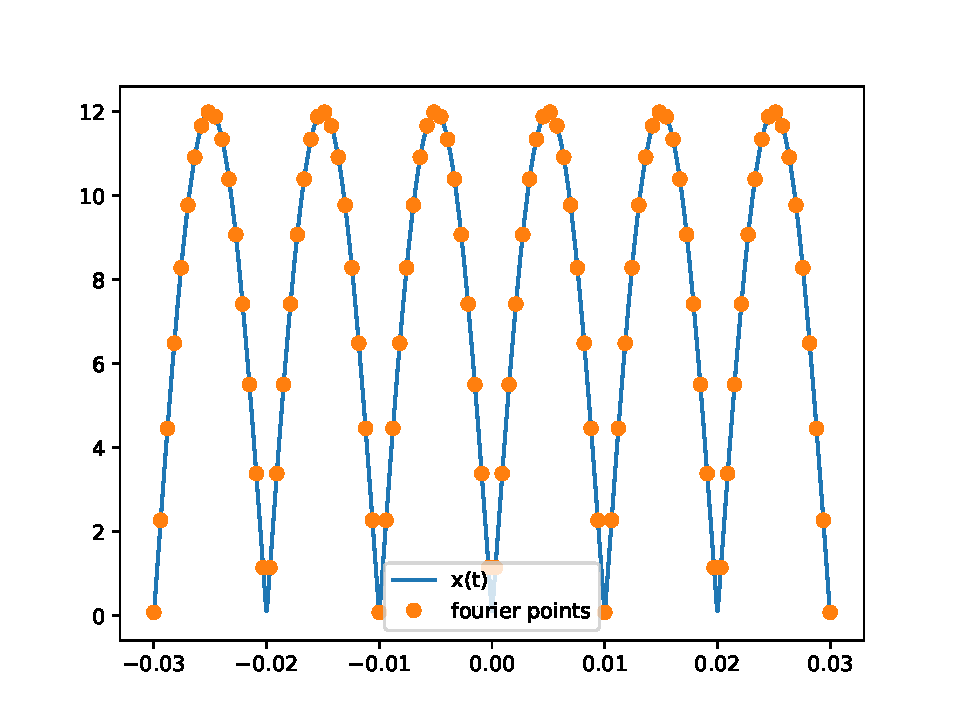
\includegraphics[width=\columnwidth]{figs/2_3.pdf}
	\caption{}
\end{figure}


\item Show that 
\begin{align}
	x(t) = \sum_{k = 0}^{\infty}\brak{a_k\cos{2\pi jkf_0 t}+b_k\sin{2\pi jkf_0 t}}
\label{eq:one-Z-real}
\end{align}
and obtain the formulae for $a_k$ and $b_k$.\\
\solution
\begin{align}
	&x(t) = \sum_{k = -\infty}^{\infty}c_ke^{2 \pi j kf_0 t} \\
	&x(t) = \sum_{k = -\infty}^{-1} c_k e^{2 \pi j kf_0 t} + c_0 + \sum_{k = 1}^{\infty} c_k e^{2 \pi j kf_0 t}
\end{align}
Replacing $k$ with $-k$ in the first summation, we have 
\begin{align}
	&x(t) = \sum_{k = 1}^{\infty} c_{-k} e^{2 \pi j -k f_0 t} + c_0 + \sum_{k = 1}^{\infty} c_k e^{2 \pi j kf_0 t} \\
	&x(t) = c_0 + \sum_{k = 1}^{\infty} \brak{c_k e^{2 \pi j kf_0 t} + c_{-k} e^{-2 \pi jk f_0 t}}
\end{align}
\begin{multline}
	x(t) = c_0 + \sum_{k = 1}^{\infty} \brak{c_k + c_{-k}} \cos{\brak{2 \pi j kf_0 t}} \\ + \text{j} \sum_{k = 1}^{\infty} \brak{c_k - c_{-k}} \sin{\brak{2 \pi j k f_0 t}}
\end{multline}
The coefficients $a_k, b_k$ can be expressed as follows, 
\begin{align}
a_k = 
	\begin{cases}
		\quad c_0 \hspace{2.3em} k = 0 \\
		c_k + c_{-k} \quad k > 0
	\end{cases}
\end{align}
\begin{align}
b_k = 
	\begin{cases}
		\quad 0 \hspace{2.6em} k = 0 \\
	    	c_k - c_{-k} \quad k > 0
	\end{cases}
\end{align}


\item Find $a_k$ and $b_k$ for 
	\eqref{eq:10-orig-diff-def} \\
\solution
Using \eqref{eq:c_k} in the above coefficient expressions, we have 
\begin{align}
&c_0 = \frac{2 A_0}{\pi} \\
&c_k + c_{-k} = \frac{2 A_0}{\pi \brak{1 - k^2}} + \frac{2 A_0}{\pi \brak{1 - (-k)^2}}
\end{align}

\begin{align}
&a_k = 
	\begin{cases}
		\quad \cfrac{2 A_0}{\pi} \hspace{2.3em} k = 0 \vspace{1em} \\ \, \, \cfrac{4 A_0}{\pi \brak{1 - k^2}} \hspace{1.5em} k > 0
	\end{cases} \\ 
	\vspace{2em} &b_k = 0 \hspace{1em} k \geq 0
\label{eq:ak_bk}
\end{align}


\item Verify 
\eqref{eq:one-Z-real}
using python. \\
\solution
Download the following Python code for verifying the plot of Fourier series with coefficients obtained in \eqref{eq:ak_bk}.
\begin{figure}[!ht]
	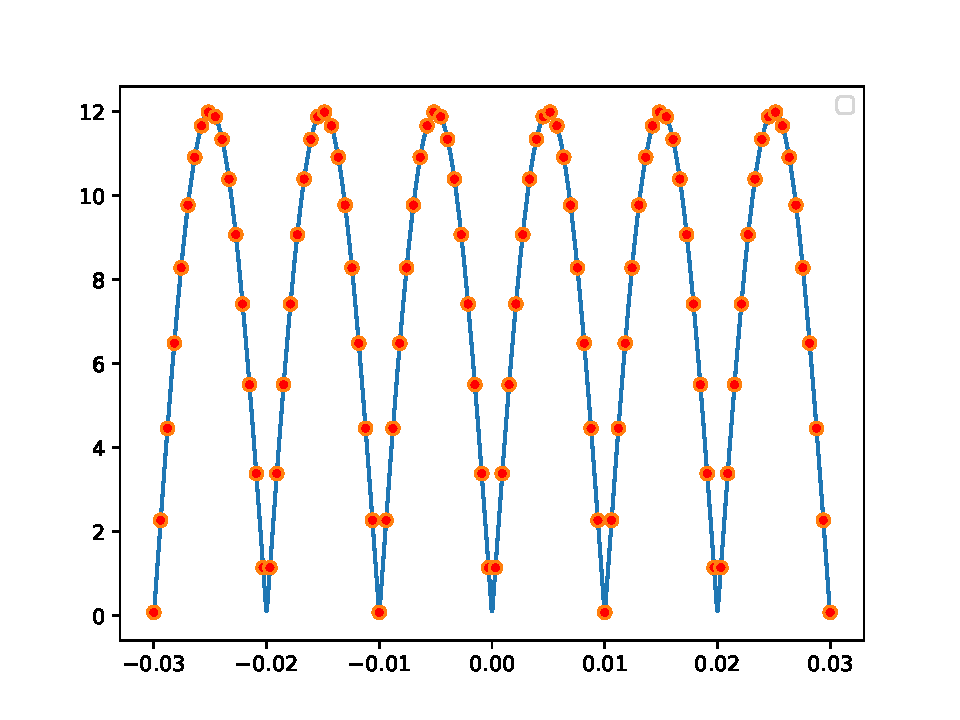
\includegraphics[width=\columnwidth]{figs/2_6.pdf}
	\caption{Fourier Series with coefficients}
\end{figure}
\end{enumerate}

\section{Fourier Transform}
\begin{enumerate}[label=\thesection.\arabic*
,ref=\thesection.\theenumi]

\item 
\begin{align}
&\delta(t)=0, \quad t\neq0
\\
&\int_{-\infty}^{\infty}\delta(t) \, dt= 1
\label{eq:delta}
\end{align}
\item The Fourier Transform of $g(t)$ is
\begin{align}
G(f)=\int_{-\infty}^{\infty}g(t)e^{-2\pi jft}\,dt
\label{eq:fourier}
\end{align}


\item Show that 
\begin{align}
g(t-t_0)&\system{F}G(f)e^{-2\pi jft_0}
\end{align}\\
\solution
Applying Fourier transform to \\ $g(t - t_0)$, we obtain
\begin{align}
	&\mathcal{F}\brak{g(t - t_0)} = \int_{-\infty}^{\infty}g(t - t_0)e^{-2\pi jft}\,dt \\
	&\mathcal{F}\brak{g(t - t_0)} = e^{-2 \pi jf t_0} \int_{-\infty}^{\infty}g(t - t_0)e^{-2\pi jf\brak{t - t_0}} \,dt 
\end{align}
Using definition of Fourier transform from \eqref{eq:fourier}, we have 
\begin{align}
	\mathcal{F}\brak{g(t - t_0)} = G(f)e^{-2\pi jft_0}
\end{align}


\item Show that 
\begin{align}
 G(t)&\system{F}g(-f)
\end{align}
\solution
From the definition of Inverse Fourier transform, we have 
\begin{align} 
	&g(t) = \int_{-\infty}^{\infty} G(f) e^{2 \pi jft} \text{df}
	\label{eq:inv_fourier}
\end{align}
In \eqref{eq:inv_fourier}, substituting $f \rightarrow t$ and $t \rightarrow -f$,
\begin{align}
	&g(-f) = \int_{-\infty}^{\infty} G(t) e^{-2 \pi jft} \text{dt}
\end{align}
From \eqref{eq:fourier}, we can conclude that 
\begin{equation}
	\mathcal{F}\brak{G(t)} = g(-f)
\end{equation}


\item $\delta(t)\system{F}?$ \\
\solution
Using the following property of $\delta$ function, 
\begin{align}
	f(x) \delta(x - a) = f(a) \delta(x-a)
\end{align}
From \eqref{eq:fourier}, we have 
\begin{align}
	&\int_{-\infty}^{\infty} \delta(t - 0) e^{-2 \pi jft} \text{dt} \\
	&= \int_{-\infty}^{\infty} \delta(t) e^{0} \text{dt} = \int_{-\infty}^{\infty} \delta(t) \text{dt} 
\end{align}
So, the Fourier transform of the $\delta$-function is 
\begin{equation}
	\delta(t) \system{F} 1
\end{equation}


\item $e^{-j2\pi f_0t}\system{F}?$ \\
\solution
From \eqref{eq:fourier}, we have 
\begin{align}
	\mathcal{F}\brak{e^{-j2\pi f_0t}}&=\int_{-\infty}^{\infty} e^{-2 \pi j f_0 t} e^{-2 \pi jft} \text{dt}\\
	&=\int_{-\infty}^{\infty} e^{-2 \pi j \brak{f + f_0} t} \text{dt}
\end{align}
\begin{align}
	1 &\system{F} \delta\brak{-f} \\
	\implies &\int_{-\infty}^{\infty} e^{-2 \pi jft} \text{dt} = \delta\brak{-f} \\
	\implies &\int_{-\infty}^{\infty} e^{-2 \pi j\brak{f + f_0} t} \text{dt} = \delta\brak{-(f + f_0)} \\
		 &e^{-2 \pi j f_0 t} \system{F} \delta\brak{f + f_0}
\end{align}


\item $\cos(2\pi f_0t)\system{F}?$ \\
\solution Using the linearity of the Fourier 
Transform and \eqref{eq:fourier},
\begin{align}
	\cos\brak{2\pi f_0t} &= \frac{1}{2} \brak{e^{2\pi j f_0t} + e^{-2\pi j f_0t}} \\
	e^{2 \pi j f_0 t} &\system{F}\delta\brak{f+f_0} \\
	e^{-2 \pi j f_0 t} &\system{F}\delta\brak{f-f_0} \\
	\cos\brak{2 \pi f_0t} &\system{F}\frac{1}{2} \bigl(\delta\brak{f + f_0} + \delta\brak{f - f_0}\bigr)
\end{align}


\item Find the Fourier Transform of $x(t)$ and plot it. Verify using python \\\solution
\begin{align}
&x(t) = A_0 \abs{\sin{2 \pi f_0 t}} \\
&\mathcal{F}\brak{x(t)} = \int_{-\infty}^{\infty} A_0 \abs{\sin{2 \pi f_0 t}} e^{-2 \pi jft} \text{dt} \\
&= \int_{0}^{\infty} A_0 \sin{\brak{2 \pi f_0 t}} e^{-2 \pi jft} \text{dt} + A\\
&= \frac{A_0}{2j} \int_{0}^{\infty} A_0 \brak{e^{2 \pi jf_0t} - e^{-2 \pi jf_0t}}e^{-2 \pi jft} \text{dt} + A \\
&= \frac{A_0}{2j} \int_{0}^{\infty} e^{2 \pi j (f_0 - f) t} \text{dt} - \int_{0}^{\infty} e^{-2 \pi j (f_0 + f) t} \text{dt} + A \\
&= -\frac{A_0}{4 j^2 \pi (f_0 - f)} - \frac{A_0}{4 j^2 \pi (f_0 + f)} + A \\
&= \frac{A_0}{2 \pi \brak{{f_0}^2 - f^2}} + A
\end{align}
Calculating the value of A, 
\begin{align}
	&A = \int_{-\infty}^{0} -A_0 \sin{\brak{2 \pi f_0 t}} e^{-2 \pi jft} \text{dt} \\
	&A = -\frac{A_0}{2j} \, \Biggl[ \int_{-\infty}^{0} e^{2 \pi j (f_0 - f) t} \text{dt} - \int_{-\infty}^{0} e^{-2 \pi j (f_0 + f) t} \text{dt} \Biggr] \\
	&A = -\frac{A_0}{2j} \, \Biggl( \frac{1}{2 \pi j (f_0 - f)} + \frac{1}{2 \pi j (f_0 + f)} \Biggr) \\
	&A = \frac{A_0}{2 \pi \brak{f_{0}^2 - f^2}}
\end{align}
\begin{align}
	A_0 \abs{\sin{2 \pi f_0 t}} \system{F} \frac{A_0}{\pi \brak{f_{0}^2 - f^2}}
\end{align}
\begin{figure}[!ht]
	\centering
	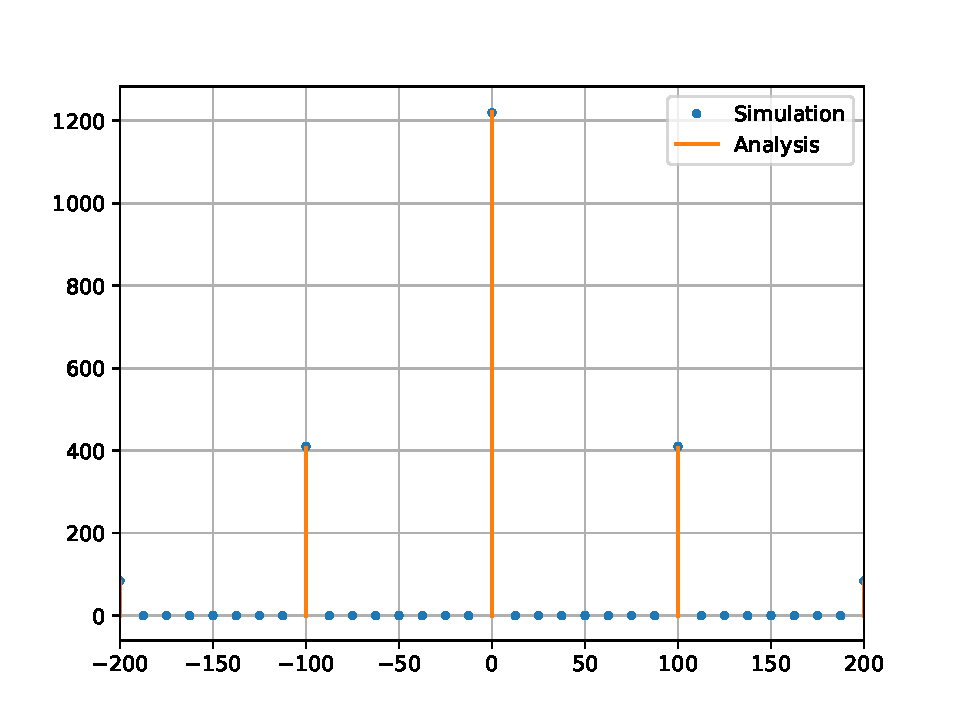
\includegraphics[width=\columnwidth]{figs/3_8.pdf}
\end{figure}
\vspace{5mm}


\item Show that 
\begin{align}
\rect{t} \system{F} \sinc{t}
\end{align}
Verify using python. \\
\solution
solution We write
\begin{align}
	&\mathcal{F}\brak{\rect{t}} = \int_{-\infty}^{\infty}\rect{t}e^{-2\pi jft}\, dt \\
            &=\int_{-\frac{1}{2}}^{\frac{1}{2}}e^{-2\pi jft}\, dt \\
            &=\frac{e^{\pi jf} - e^{-\pi jf}}{2\pi jf} \\
	    &= \frac{\sin{\pi f}}{\pi f} = \sinc{f}
            \label{eq:fourier-rect}
\end{align}
Verifying using plot in Python,


\item 
$\sinc{t}\system{F}?$. Verify using python. \\
\solution From \eqref{eq:inv_fourier}, we have 
\begin{align}
	\sinc{t}\system{F}\rect {-f}
    \label{eq:fourier-sinc}
\end{align}
Since $\rect{f}$ is an even function, we have 
\begin{align}
	\sinc{t} \system{F} \rect{f}
\end{align}
\begin{figure}
	\centering
	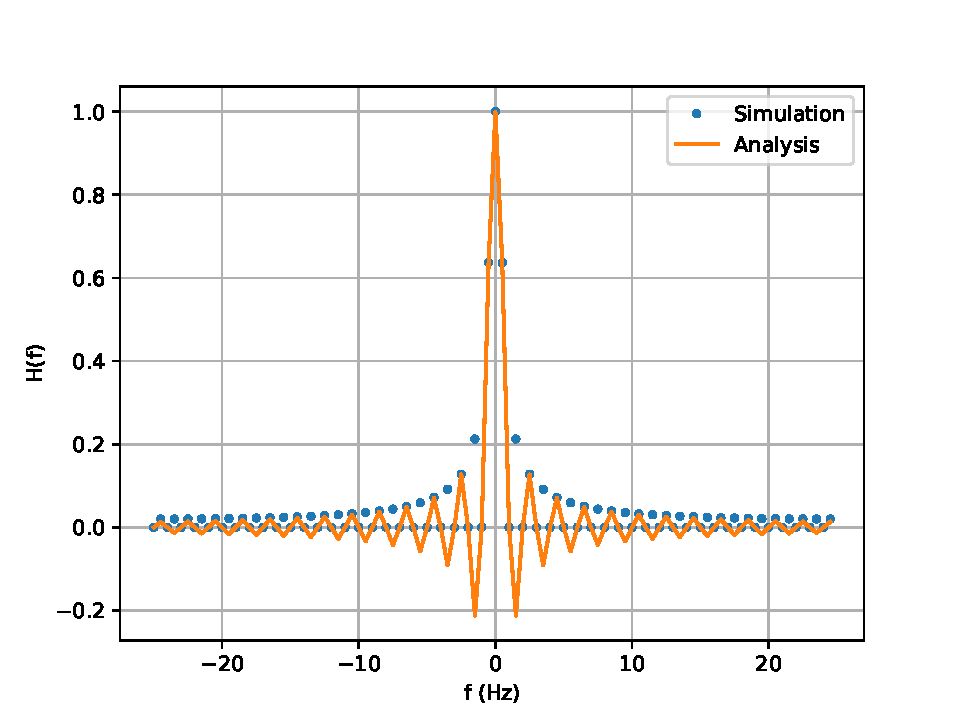
\includegraphics[width=\columnwidth]{figs/3_9.pdf}
\end{figure}
\begin{figure}[!ht]
	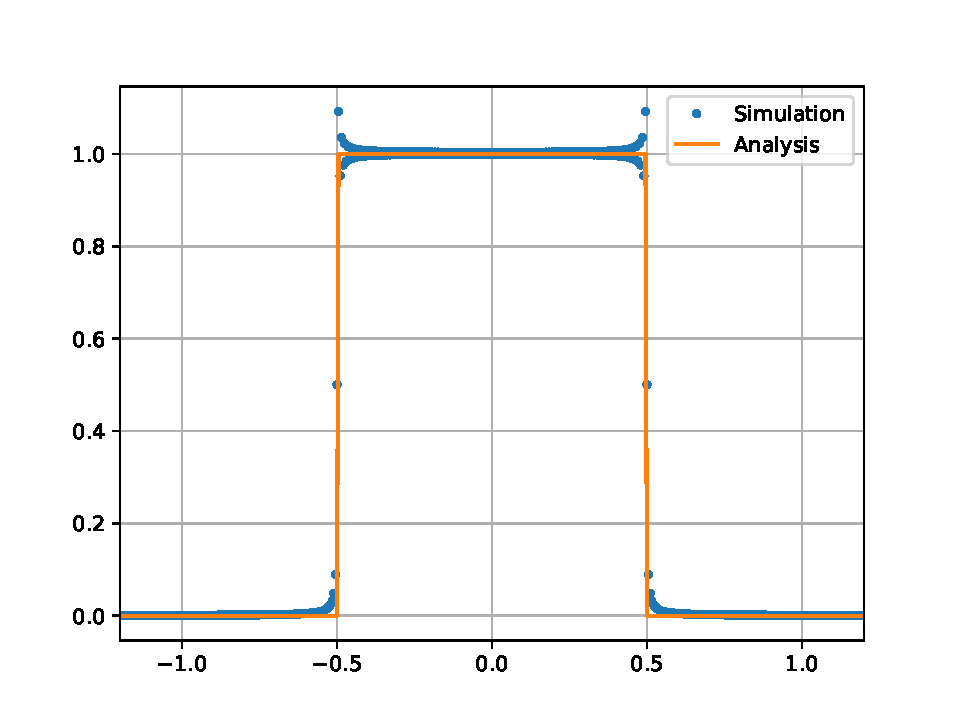
\includegraphics[width=\columnwidth]{figs/3_10.pdf}
\end{figure}
\end{enumerate}


\section{Filter}
\begin{enumerate}[label=\thesection.\arabic*
,ref=\thesection.\theenumi]
\item Find $H(f)$ which transforms $x(t)$ to DC 5V. \\
\solution The function $H(f)$ is a low pass filter which filters out
even harmonics and leaves the zero frequency component behind. \\ From the previous Fourier transform, we can see that the $\rect{t}$ function represents an ideal low pass filter. Suppose the cutoff frequency is $f_c = 50$ Hz, then
\begin{align}
	H(f) = \rect{\frac{f}{2f_c}} =
	\begin{cases}
		1 & \abs{f} < f_c \\
		0 & \textrm{otherwise}
	\end{cases}
\end{align}
Multiplying by a scaling factor to get DC 5V,
\begin{align}
	H(f) = \frac{\pi V_0}{2A_0}\rect{\frac{f}{2f_c}}
	\label{eq:H_f}
\end{align}
where $V_0 = 5$ V.


\item Find $h(t)$. \\
\solution Suppose $g(t)\system{F}G(f)$. Then, for some
nonzero $a \in \mathbb{R}$, let $u=at$,
\begin{align}
	g(at)&\system{F}\frac{1}{a}G\brak{\frac{f}{a}}
\end{align}
From \eqref{eq:H_f}, we have 
\begin{align}
	\implies h(t)&\system{F} \frac{\pi V_0}{2A_0}\rect{\frac{f}{2f_c}}\\
	h(t)&\system{F} \frac{\pi V_0 2f_c}{2A_0}  \frac{1}{2f_c}\rect{\frac{f}{2f_c}}\\
	h(t)&\system{F} \frac{2 \pi f_c V_0}{A_0}\rect{\frac{f}{2f_c}}\\
	h(t) &= \frac{2\pi V_0}{A_0}f_c\sinc{\brak{2f_ct}}
\end{align}


\item Verify your result using through convolution. \\ 
\solution 
	Fourier transform of $x(t)$ and $h(t)$ respectively is
	\begin{align}
		X(f)&=\sum_{k=-\infty}^{\infty} \frac{2A_0}{\pi} \frac{\delta\brak{f-2kf_0}}{1-4k^2}\\
		H(f)&=\frac{\pi V_0}{2A_0}\rect{\frac{f}{2f_c}}\\
		X(f) \times H(f)&=\sum_{k=-\infty}^{\infty} V_0 \frac{\delta\brak{f-2kf_0}}{1-4k^2} \rect{\frac{f}{2f_c}}\\
		X(f)\times H(f)&=\sum_{k=0}^{0} V_0 \frac{\delta\brak{f-2kf_0}}{1-4k^2}
	\end{align} 
	Hence,
	\begin{align}
		X(f)\times H(f)&=V_0 \frac{\delta\brak{f}}{1-4 \times 0}\\
		X(f)\times H(f)&=V_0 \delta\brak{f}
	\end{align} 
\begin{align}
	V_0 \delta\brak{t} \stackrel{\mathcal{F}^{-1}}{\longleftrightarrow} V_0\times 1	\\
\implies H(t) * x(t)=V_0
\end{align}
\begin{figure}[!ht]
	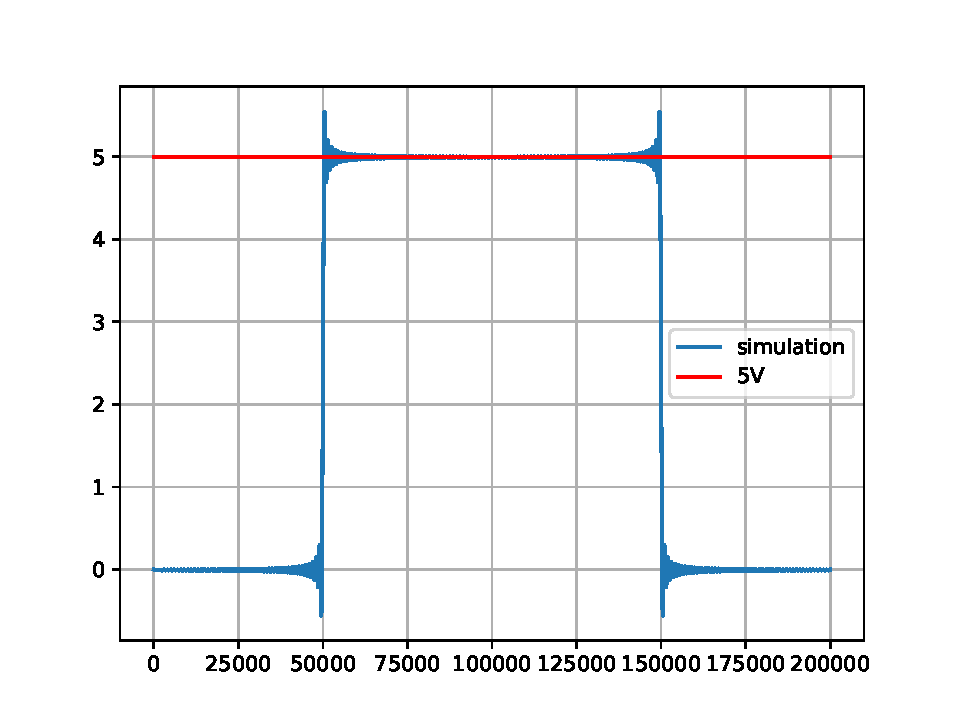
\includegraphics[width=0.9\columnwidth]{figs/4_3.pdf}
\end{figure}
\end{enumerate}
\vfill{}

\section{Filter Design}
\begin{enumerate}[label=\thesection.\arabic*
,ref=\thesection.\theenumi]
\item Design a Butterworth filter for $H(f)$.\\
\solution
Butterworth filters are designed to have a frequency response as flat as possible in the passband. Here, we design a low-pass filter of order $n$. As the order of filter increases, excessive ripple is produced in the passband. \\
Generalized form of frequency response for $n^{\text{th}}$ order Butterworth low-pass filter is 
\begin{align}
	H(f) = \frac{1}{\sqrt{ 1 + \brak{\frac{f}{f_c}}^{2n}}}
\end{align}
\begin{itemize}
	\item n is the order 
	\item w = operating frequency 
	\item $w_c =$ cutoff frequency 
	\item $\epsilon =$ maximum passband gain 
\end{itemize}
To find the order of the filter, we consider the following values 
\begin{itemize}
	\item Passband frequency = 50Hz
	\item Stopband frequency = 100Hz
	\item Attenuation between -1 dB and -5 dB
\end{itemize}
\begin{align}
	A_p &= 10 \log_{10}\abs{H_n(f_p)}^2 \\
	&= -10\log_{10}\brak{1+\brak{\frac{f_p}{f_c}}^{2n}} \\
	A_s &= -10\log_{10}\brak{1+\brak{\frac{f_s}{f_c}}^{2n}} \\
	\implies n &=\frac{\log\brak{\frac{10^{-\frac{A_p}{10}}-1}{ 10^{-\frac{A_s}{10}}-1}}}{2 \log \brak{\frac{f_p}{f_s}}} \approx 1.53
\end{align}
Hence, we choose a $2^{\mathrm{nd}}$ order Butterworth filter with
\begin{align}
	f_c = \frac{f_p}{\brak{10^{-\frac{A_p}{10}}-1}^{\frac{1}{2n}}} \approx 77.74Hz
\end{align}


\item Design a Chebyschev filter for $H(f)$.\\
\solution
Chebyshev filters are used for distinct frequencies of one band from another. They are carried out by recursion rather than convolution. \\
Frequency response of Type-1 Chebyshev filter is given by
\begin{align}
	\abs{H_n(f)} =\frac{1}{\sqrt{1+\epsilon^{2}T_{n}^2\brak{\frac{f}{f_c}}}}
\end{align}
\begin{itemize}
	\item $\epsilon$ = ripple factor
	\item $f_c$ = cutoff frequency 
	\item $T_n$ = Chebyshev polynomial of $n^{th}$ order
\end{itemize}
Assuming the same parameters as before along with a ripple of $0.1 Db$, we get
\begin{align}
	\epsilon = \sqrt{10^{\frac{\delta}{10}} - 1} \approx 0.15
\end{align}
Also, assume that $f_c = f_p \implies \frac{f_s}{f_c} > 1$
\begin{align}
	&A_s = -10\log_{10}\brak{1+\epsilon^{2}T_{n}^2\brak{\frac{f_s}{f_c}}} \\
	\implies &T_{n}\brak{\frac{f_s}{f_c}} = \frac{\sqrt{10^{-\frac{A_s}{10}} - 1}}{\epsilon} \\
	\implies &\cosh\brak{n\cosh^{-1}\brak{\frac{f_s}{f_c}}} = \frac{\sqrt{10^{-\frac{A_s}{10}} - 1}}{\epsilon} 
\end{align}
Thus
\begin{align}
	n = \frac{\cosh^{-1}\brak{\frac{\sqrt{10^{-\frac{A_s}{10}} - 1}}{\epsilon} }}{\cosh^{-1}\brak{\frac{f_s}{f_c}}} \approx 2.26
\end{align}
Hence, we choose a $3^{\mathrm{rd}}$ order Chebyshev filter.


\item Design a circuit for your Butterworth filter\\	
\solution Using the table of normalized Butterworth coefficients, we can see that for a $2^{\mathrm{nd}}$ order Butterworth filter
\begin{align}
	C_1 &= 1.4142 F \\
	L_2 &= 1.4142 H
\end{align}
On denormalizing these values, we get
\begin{align}
	C_1' &= \frac{C_1}{2\pi f_c} = 2.89 mF \\
	L_2' &= \frac{L_2}{2\pi f_c} = 2.89 mH
\end{align}
\begin{figure}[!ht]
\centering
\begin{circuitikz} 
\draw (0,0) to[short, o-o] (4,0);
\draw (1,0) to[C, l=2.89 mF] (1,2);
\draw (0,2) to [short, o-] (1,2) 
	to [L, l=2.89 mH] (3.5,2) 
        -- (4,2) to[short, -o] (4,2);      
\end{circuitikz}
\caption{$2^{\mathrm{nd}}$ order Butterworth filter circuit}
\label{ckt:butter}
\end{figure}


\item Design a circuit for your Chebyschev filter \\
\solution Using the table of normalized Chebyshev coefficients, we can see that for a $3^{\mathrm{rd}}$ order Chebyshev filter
\begin{align}
	C_1 &= 1.432 F \\
	L_2 &= 1.5937 H \\
	C_3 &= 1.4328 F
\end{align}
On denormalizing these values, we get
\begin{align}
	C_1' &= \frac{C_1}{2\pi f_c} = 4.56 mF \\
	L_2' &= \frac{L_2}{2\pi f_c} = 5.07 mH \\
	C_3' &= \frac{C_3}{2\pi f_c} = 4.56 mF
\end{align}
\begin{figure}[!ht]
\centering
\begin{circuitikz} 
\draw (0,0) to[short, o-o] (5,0);
\draw (0,2) to [short, o-] (1,2) 
     		to [L, l=5.07 mH] (3.5,2) 
        	-- (5,2) to[short, -o] (5,2);
\draw (1,0) to[C, l=4.56 mF] (1,2);
\draw (3.5,0) to[C, l=4.56 mF] (3.5,2);
\end{circuitikz}
\caption{$3^{\mathrm{rd}}$ order Chebyshev filter circuit}
\label{ckt:cheby}
\end{figure}
\end{enumerate}
\end{document}

%
% 
%\solution
%\begin{align}
%	x(t) &= \sum_{k = -\infty}^{\infty}c_ke^{2\pi j kf_0 (t)} 
%\end{align}
%Replacing $k \longrightarrow -k$, we have 
%\begin{align}
%	&= \sum_{k = -\infty}^{\infty}c_{-k}e^{2\pi j (-k) f_0 t} \\
%	&= \sum_{k = -\infty}^{\infty}c_{-k}e^{2\pi j kf_0 t} 
%\end{align}
%So, we have the relation $c_k = c_{-k}$
%
%Rewriting the summation as follows, 
%\begin{align}
%	x(t) = &c_0 + \sum_{k = 1}^{\infty} c_k e^{2\pi j k f_0 t} \\
%	x(t) = &c_0 + \sum_{k = 1}^{\infty} c_k \cos{\brak{2\pi k f_0 t}} + \\ &\sum_{k = 1}^{\infty} c_k j \sin{\brak{2\pi k f_0 t}} 
%\end{align}

%Taking integral over one time period on both sides, we have 
%\begin{align}
%	\int_{0}^{T} x(t) dt &= \int_{0}^{T} c_0 + \int_{0}^{T} \sum_{k = 1}^{\infty} c_k \cos{\brak{2\pi k f_0 t}} dt \\ &+ \int_{0}^{T}\sum_{k = 1}^{\infty} c_k j \sin{\brak{2\pi k f_0 t}} dt 
%\end{align}
%
%Using the following properties
%\begin{align}
%	\int_{0}^{T} \sin{\brak{2\pi k f_0 t}} dt = 0 \\
%	\int_{0}^{T} \cos{\brak{2\pi k f_0 t}} dt = 0
%\end{align}
%
%We have the following equation, 
%\begin{align}
%	\i%t_{0}^{T} x(t) dt = c_0 \int_{0}^{T} dt \\
%	c_0 = \frac{1}{T} \int_{0}^{T} x(t) dt
%\end{align}
%
%Multiplying the equation with $\cos{2\pi k^{'} f_0 t}$ \\ and taking integral over one time period, we have
%
%\begin{align}
%\int_{0}^{T} \cos{\brak{2 \pi k_i f_0 t}} \cos{\brak{2 \pi k f_0 t}} = \\ 
%\begin{cases}
%	0 \,  \text{if} \quad k_i = k_0 \\
%	\frac{T}{2} \, \text{if} \quad k_1 \neq k_0
%\end{cases}
%\end{align}
%
%Hence, we have 
%\begin{align}
%	\int_{0}^{T} x(t) \cos{\brak{2 \pi k^{'} f_0 t}} = c_k \frac{T}{2}
%\end{align}
%
%
%
